%ablaufplan des Projekts
\section{Ablaufplan}
In diesem Kapitel wird der Ablaufplan des Projekts beschrieben
\subsection{Phase 1: Pflichtenheft}
\textbf{Ziel:} Erstellung des Pflichtenhefts \newline
\textbf{Phasenverantwortlicher:} Laurenz Thiel \newline
\textbf{Abgabe:} 29 November 2015 \newline
\textbf{Artefakt:} Pflichtenheft \newline
Im Pflichtenheft werden die Anforderungen, Funktionen, die grobe Benutzerschnittstellen, Systemmodelle und Testszenarios für das Programm erstellt. Des weiteren werden Sachen wie die Entwicklungsumgebung und mögliche Hardware- und Softwarevoraussetzungen festgehalten. Das Pflichtenheft soll präzise, vollständig und konsistent sein.

\subsection{Phase 2: Entwurf}
\textbf{Ziel:} Erstellung des Entwurfs \newline
\textbf{Phasenverantwortlicher:} Tim Brodbeck \newline
\textbf{Abgabe:} 10 Januar 2016 \newline
\textbf{Artefakt:} UML-Diagramm des Entwurfs \newline
Im Entwurf wird das Design der Software festgelegt. Es wird die Klassenstruktur, die Beziehungen zwischen den Klassen und die Klassenschnittstellen definiert. Des weiteren werden Klassendiagramme erstellt und zusätzlich können noch Sequenz- und Zustandsdiagramme erstellt werden. Es sollten Entwurfsmuster aus der Softwaretechnik zum Einsatz kommen. Es soll auf das Geheimnisprinzip, schwache Kopplung, hohe Kohäsion, Lokalitätsprinzip und Wiederverwendbarkeit von Klassen/Subsystemen geachtet werden

\subsection{Phase 3: Implementierung}
\textbf{Ziel:} Schreiben des Quellcodes \newline
\textbf{Phasenverantwortlicher:} Jens Manig, Nathanael Schneider  \newline
\textbf{Abgabe:} 7 Februar 2016 \newline
\textbf{Artefakt:} Quellcode \newline
In dieser Phase wird das Programm implementiert. Es werden die Klassen und deren Methoden aus der Entwurfsphase implementiert.

\subsection{Phase 4: Qualitätssicherung}
\textbf{Ziel:} Testen des Systems und schreiben von Testberichten \newline
\textbf{Phasenverantwortlicher:} Stefan Wolf  \newline
\textbf{Abgabe:} 6 März 2016 \newline
\textbf{Artefakt:} Tests \newline
Es werden verschiedene Tests(z.B. funktionale Komponententests, Überdeckungstests) durchgeführt und Testberichte geschrieben. Es werden ebenfalls die, im Pflichtenheft beschriebenen, Testfälle getestet. Ebenfalls wird die Robustheit des Systems überprüft.

\subsection{Phase 5: Abschlusspräsentation}
\textbf{Ziel:} Vorbereiten der Abschlusspräsentation \newline
\textbf{Phasenverantwortlicher:} Grigori Schapoval  \newline
\textbf{Abgabe:} 20 März 2016 \newline
\textbf{Artefakt:} Präsentation \newline
Es wird die Abschlusspräsentation vorbereitet, in der dass Produkt vorgestellt wird. \newline
\newline
\newline
Hier der Ablauf als Diagramm \newline
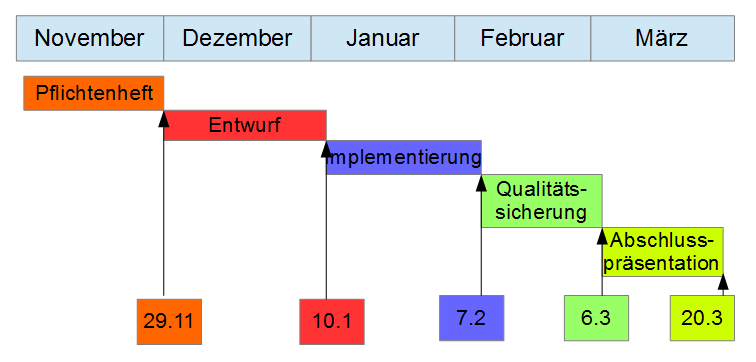
\includegraphics{img/ablauf.png}